\documentclass[twocolumn]{aastex61}
\usepackage{bm}
\usepackage{amsmath,amsfonts,amssymb}
\usepackage{color}
\usepackage{comment}

\newcommand\teff{T_{\rm eff}}
\newcommand\logg{\log{g}}
\newcommand\feh{[\rm{Fe}/\rm{H}]}

\newcommand{\project}[1]{\textsl{#1}}
\newcommand{\package}[1]{\texttt{#1}}
\newcommand{\acronym}[1]{{\small{#1}}}

\newcommand{\Gaia}{\project{Gaia}}
\newcommand{\gaia}{\project{gaia}}
\newcommand{\Galah}{\project{Galah}}
\newcommand{\GALAH}{\project{GALAH}}
\newcommand{\todo}[1]{\textcolor{red}{#1}}


\newcommand{\vect}[1]{\boldsymbol{\mathbf{#1}}}
\renewcommand{\vec}[1]{\vect{#1}}

\newcommand{\weight}{\pi}
\newcommand{\data}{\textbf{Y}}
\newcommand{\vecdata}{\vec\data}

\newcommand{\nextstep}{^\textrm{(t+1)}}
\newcommand{\thisstep}{^\textrm{(t)}}
\newcommand{\transpose}{^\intercal}
\newcommand{\eye}{\textbf{I}}

\newcommand{\factorloads}{\textbf{L}}
\newcommand{\factorscores}{\textbf{S}}
\newcommand{\specificvariance}{\vec{D}}

\newcommand{\scoremeans}{\vec\xi}
\newcommand{\scorecovs}{\vec\Omega}

\newcommand{\NumData}{N}
\newcommand{\NumDimensions}{D}
\newcommand{\numdata}{n}
\newcommand{\numdimensions}{d}
\newcommand{\NumLatentFactors}{J}
\newcommand{\numlatentfactors}{j}
\newcommand{\NumComponents}{K}
\newcommand{\numcomponents}{k}




\received{2018 XX XX}
\revised{2018 XX XX}
\accepted{2018 XX XX}

\newcommand{\vcpath}{vc.tex}

\IfFileExists{\vcpath}{\input{\vcpath}}{
	\newcommand{\giturl}{UNKNOWN}
	\newcommand{\gitslug}{UNKNOWN}
	\newcommand{\githash}{UNKNOWN}
	\newcommand{\gitdate}{UNKNOWN}
	\newcommand{\gitauthor}{UNKNOWN}
}



\submitjournal{AAS Journals}

\shorttitle{Statistically consistent chemical tagging}
\shortauthors{Casey et al.}

\begin{document}

\title{A statistically consistent approach to chemical tagging}

\correspondingauthor{Andrew R. Casey}
\email{andrew.casey@monash.edu}

\author[0000-0003-0174-0564]{Andrew R. Casey}
\affiliation{School of Physics \& Astronomy, 
			 Monash University,
			 Wellington Rd, Clayton 3800, Victoria, Australia}
\affiliation{Faculty of Information Technology, 
			 Monash University, 
			 Wellington Rd, Clayton 3800, Victoria, Australia}
			 
\author{John Lattanzio}
\affiliation{School of Physics \& Astronomy, 
			 Monash University,
			 Wellington Rd, Clayton 3800, Victoria, Australia}

\author{Aldeida Aleti}
\affiliation{Faculty of Information Technology, 
			 Monash University, 
			 Wellington Rd, Clayton 3800, Victoria, Australia}

\author{David Dowe}
\affiliation{Faculty of Information Technology, 
			 Monash University, 
			 Wellington Rd, Clayton 3800, Victoria, Australia}

\author{the GALAH team}


\begin{abstract}
Chemical tagging promises to distinguish unique star formation sites based on the
present day photospheric abundances of stars.  It is not known how effective this
will be.  Clustering techniques used for chemical tagging  assume statistical 
independence between abundances. Theory and observations agree that this assumption
is incorrect: some elemental abundances are produced through multiple nucleosynthetic
processes, and most nucleosynthetic processes generates multiple chemical abundances.
Here we introduce a statistically consistent approach to chemical tagging, where we
simultaneously infer the nucleosynthetic processes that produce chemical abundances,
and we perform clustering in this lower dimensional latent space. \todo{we use galah}
\todo{scales iwth data}
\end{abstract}


\keywords{methods: statistical}

\section{Introduction} \label{sec:intro}

\begin{itemize}
	\item Chemical tagging
	\item Limits on the efficacy of chemical tagging
	\item Clustering vs common traits
	\item Dimensionality of data space
\end{itemize}



The \Galah\ survey \citep{DaSilva:2015} is a stellar spectroscopic survey 
that uses the High Efficiency and Resolution Multi-Element 
Spectrograph \citep[HERMES][]{Sheinis:2016} on the Australian Astronomical Telescope (AAT).
The survey will observe up to $10^6$ stars in the Milky Way, and
measure up to 30 chemical abundances for each star. This includes
light odd-Z elements (e.g., Na, K), elements produced through
alpha-particle capture (e.g., Mg, Ca, Ti), and elements produced
through the slow (e.g., Ba) and rapid neutron-capture process
(e.g., Eu). These data provide an unparalleled view on the production
of chemical elements in the Milky Way.

\section{Methods} \label{sec:methods}

%Factor analysis is a statistical method used to describe variability among observed, correlated variables in terms of a potentially lower number of unobserved variables called factors.

Factor analysis is a common statistical approach for describing correlated 
observations with a lower number of latent variables \citep{factor-analysis}.
\todo{Analagous approaches used in astrophysics: pca, etc}.

Similarly, clustering techniques are commonly used to identify groups in 
data space. 

Here we use a combination of these methods that provides a
consistent description of the data, given the latent variables and their 
clustering in latent space. In this work the data $\vecdata$ is a 
$\NumData \times \NumDimensions$ matrix where $\NumData$ is the number of 
stars and $\NumDimensions$ is the number of chemical abundances measured 
for each star. We assume a
generative model for the data 
\begin{equation}
	\vecdata = \factorloads\factorscores + \vec{e}
	\label{eq:generative-model}
\end{equation}

\noindent{}where $\factorloads$ is a $\NumLatentFactors \times \NumDimensions$ matrix of factor
loads that is common to all data points, and the factor scores for
the $\numdata$th data point
\begin{equation}
	\factorscores_\numdata \sim \mathcal{N}(\vec\xi_\numcomponents, \vec\Omega_\numcomponents)
\end{equation}
\noindent{}are drawn from the $\numcomponents$th multivariate  normal distribution.
The factor scores for all data points $\factorscores$ is then a 
$\NumData \times \NumLatentFactors$ matrix.
 We assume $\vec{e} \sim \mathcal{N}\left(\vec{0}, \eye\specificvariance\right)$
is independent of the latent space, and $\specificvariance$ is a
diagonal matrix of $\NumDimensions$ entries. In Appendix~\ref{app:symbols}
we list all mathematical symbols used in this work and their description.
In this model each data point can be represented as being drawn
from a mixture of multivariate normal components, except the components
are \emph{clustered in the latent space} $\factorscores$ and projected
into the data space by the factor loads $\factorloads$. 


We assume that the latent space is lower dimensionality than the
data space (e.g., $\NumLatentFactors < \NumDimensions$).
Within the context of stellar abundances, the factor loads
$\factorloads$ can be thought of as the \emph{typical} yields
of nucleosynthetic
events (e.g., $s$-process production from AGB stars), and the
factor scores are analogous to the relative counts of those 
nucleosynthetic events. The clustering in factor scores
achieves the same as a clustering procedure in data space,
except we simultaneously estimate the latent processes that are
common to all stars (the so-called factor loads, analogous to 
nucleosynthetic yields). Within this framework a rare nucleosynthetic event
can still be described as a `factor load' $\factorloads_\numlatentfactors$, 
but its rarity would be represented by associated factor
scores being zero for most stars and thus have negligible contribution
to the observed abundances. In practice the factor loads can only be 
identified up to orthogonality and cannot be expressly interpreted as
nucleosynthetic yields because they have limited physical meaning,
but this description of typical yields and relative event rates should
help build intuition for the model parameters, and provide context
within the astrophysical problem it is being applied.

\todo{this model of orthogonality takes the independence into account}

Another benefit of using a mixture of common factor analysers is
for modelling stellar chemical abundances is the scaling with
computational cost. If we considered data sets of order $3\times10^7$
entries (e.g., 30 chemical abundances for $10^6$ stars) purely as a
clustering problem, then even the most efficient clustering
algorithms would incur a significant cumulative computational 
overhead by searching the parameter space for the number of
clusters, and the optimal model parameters given that number
of components. However, because the mixture of factor analyzers
approach assumes that there is a \emph{lower dimensional latent 
space} in which the data are clustered, and that clustering is 
projected into real space by common factor loads, the 
dimensionality of the clustering problem is reduced from 
$N \times D$ to $N \times J$. This reduces computational cost through
faster execution of each E-M step, and on average fewer E-M steps
needed to reach a specified convergence threshold.

From a statistical standpoint, the primary advantage to using
a mixture of factor analysers is that we can simultaneously
estimate latent factors (e.g., infer nucleosynthetic 
yields) and perform clustering (e.g., chemical tagging) 
within a statistically consistent framework. That is to say
that we have a generative model for the data that can 
quantitatively account for nucleosynthetic yields, variations in
turbulence and gas mixing, or star formation efficiency,
%can account
%analogues of nucleosynthetic yields and star formation,
and the parameters of this model can be estimated consistently
given some data.

Without loss of generality the density of the data $\vecdata$ can be described as
\begin{equation}
	f(\vecdata; \vec\Psi) = \sum_{\numcomponents=1}^{\NumComponents}\weight_\numcomponents\phi(\vecdata;\factorloads\scoremeans_\numcomponents, \factorloads\scorecovs_\numcomponents\factorloads\transpose + \eye\specificvariance)
\end{equation}
\noindent{}given $\NumLatentFactors$ common factor loadings and $\NumComponents$ components
clustered in the latent (factor score) space. Here the parameter
vector
$\vec\Psi$ includes $\{\factorloads,\vec\pi,\scoremeans,\scorecovs,\specificvariance\}$, and $\phi(\vecdata;\vec\mu, \vec\Sigma)$
describes the density of a multivariate gaussian distribution with
mean $\vec\mu$ and covariance matrix $\vec\Sigma$,
and $\weight_\numcomponents$ describes the relative weighting of the $\numcomponents$th
component in latent space and $\sum\weight_\numcomponents = 1$.
The log likelihood is then given by
\begin{equation}
	\log\mathcal{L}(\vecdata|\vec\Psi) = \sum_{\numcomponents=1}^{\NumComponents}\log{f(\vecdata;\vec\Psi)} \quad .
\end{equation}


As mentioned previously, the model as described is indeterminate in that
there is no unique solution for the factor loads $\factorloads$ and scores
$\factorscores$. These quantities can only be determined up until 
orthogonality. However, accurate estimates of the parameter vector $\vec\Psi$
can be obtained by the expectation-maximization algorithm \citep{EM}.
%The model described by Equation~\ref{eq:generative-model} is indeterminate:
%there is no unique solution for the factor loads $\factorloads$ and scores
%$\factorscores$. However, an accurate estimate of the parameter vector $\vec\Psi$ can be obtained by the expectation-maximization algorithm \citep{EM}. 



\subsection{Initialisation}

Here we describe the default initialisation of the model parameters, which
we have found to be robust in a large set of models. Given a number of
$\NumLatentFactors$ latent factors we initialise the factor load
$\factorloads$ entries to be drawn from a uniform distribution
$\factorloads \sim \mathcal{U}\left(-1, +1\right)$ and then ensure that
the factor loads are orthogonal such that
%TODO: Should we re-write this so that we just draw from the scipy special ortho group?
\begin{equation}
	\factorloads \factorloads\transpose = \eye \quad .
\end{equation}
%        AL = linalg.cholesky(A.T @ A)
%        A = A @ linalg.solve(AL, np.eye(self.n_latent_factors))
% 	
We then initially assign each data point as belonging to one of the
$\NumComponents$ components by drawing from a multinomial distribution
and generating the responsibility matrix $\vec\tau$. Given the initial
factor loads and assignments, we then estimate the relative weights
$\vec\pi$, the mean factor scores of each component $\scoremeans$, and
the covariance matrix of factor scores of each component $\scorecovs$.
Finally, we initialise the specific variance $\specificvariance$ in each
dimension as 1. 

Other initialisation methods are available in the code 
associated with this \emph{Article}. In later Sections we show that 
the optimised model parameters are insensitive to the choice initialisation, 
up until orthogonal rotation of the latent space.


\subsection{Expectation-Maximization}

We use the expectation-maximization algorithm to estimate the model parameters.
With each expectation step we evaluate the log likelihood given the model 
parameters $\vec\Psi$, and we re-calculate the responsibility 
matrix $\vec\tau$ whose entries are the posterior probability
that the $\numdata$th data point is associated to the $\numcomponents$th component,
given the data $\vecdata$ and the current estimate of the 
parameter vector $\vec\Psi$:
\begin{equation}
	\tau_{\numdata\numcomponents} = \frac{\weight_\numcomponents\phi(\vecdata_\numdata;\factorloads\scoremeans_\numcomponents, \factorloads\scorecovs_\numcomponents\factorloads\transpose + \eye\specificvariance)}{\sum_{g=1}^{G}\weight_g\phi(\vecdata_\numdata;\factorloads\scoremeans_g, \factorloads\scorecovs_g\factorloads\transpose + \eye\specificvariance)} \quad .
\end{equation}


At the maximization step we update our estimates of the parameters,
conditioned on the data $\vecdata$ and the responsibility matrix $\vec\tau$.
First we estimate the relative weights $\vec\weight\nextstep$ given
the responsibility matrix $\vec\tau$
\begin{equation}
	\weight_\numcomponents\nextstep = \frac{1}{\NumData} \sum_{\numdata=1}^{\NumData}\tau_{\numdata\numcomponents}
	% Include proof.
\end{equation}
\noindent{}where the $\vec{X}\thisstep$ superscript refers to the current estimate of a variable
and $\vec{X}\nextstep$ refers to the updated estimate for the next iteration.
%\footnote{Here $\vec\textrm{X}\now$ refers to the current estimate of a variable $\vec\textrm{X}$ and $\vec\textrm{X}\nextstep$ refers to the updated estimate for the next iteration.}


%\noindent{}In the equations that follow (Equation~\ref{eq:X} to \ref{eq:Y})
%when we refer to any value in $\{\factorloads,\vec\pi,\scoremeans,\scorecovs,\specificvariance\}$ for brevity we are referring to the current estimate of that
%parameter (e.g., $\factorloads\thisstep$). The updated estimates are marked as such
%(e.g., $\scoremeans\nextstep$). 

The updated estimates of the mean factor scores 
$\scoremeans\nextstep$ for each component are then given by
\begin{eqnarray}
	\scoremeans_\numcomponents\nextstep = \scoremeans_\numcomponents\thisstep + \frac{\vec{G}\transpose(\vecdata\transpose - \factorloads\thisstep\scoremeans_\numcomponents\thisstep)\vec\tau_\numcomponents}{\NumData\weight_\numcomponents\nextstep}
\end{eqnarray}
\noindent{}where:
\begin{eqnarray}
	\vec{W} &=& (\scorecovs_\numcomponents\thisstep)^{-1}\eye \\
	\vec{V} &=& \left(\specificvariance\thisstep\right)^{-1} \\
	\vec{C} &=& (\vec{W} + (\factorloads\thisstep)\transpose\vec{V}\factorloads\thisstep)^{-1}\eye \\
	\vec{G} &=& \left[\vec{V} - \vec{V}\factorloads\thisstep\vec{C}\left(\vec{V}\factorloads\thisstep\right)\transpose\right]\factorloads\thisstep\scorecovs_k\thisstep \quad .
\end{eqnarray}

The covariance matrices of the components of factor scores $\scorecovs\nextstep$
are updated next,
\begin{equation}
	\scorecovs_\numcomponents\nextstep = \left(\eye - \vec{G}\transpose\factorloads\thisstep\right)\scorecovs_\numcomponents\thisstep + \frac{\vec{G}\transpose\vec{Z}\left(\vec{Z}\vec\tau_\numcomponents\transpose\right)\transpose\vec{G}}{N\weight_\numcomponents\nextstep}
\end{equation}
\noindent{}where
\begin{eqnarray}
	\vec{Z} &=& \vecdata\transpose - \factorloads\thisstep\scoremeans_\numcomponents\thisstep \quad .
\end{eqnarray}

After some linear algebra, updated estimates of the common factor loads $\factorloads\nextstep$
can be found from
\begin{equation}
	\factorloads\nextstep = \factorloads_{1}\left(\factorloads_{2}^{-1}\eye\right)
\end{equation}
\noindent{}where:
\begin{eqnarray}
	\factorloads_1 &=& \sum_{\numcomponents=1}^{\NumComponents}\left[ \vec\tau_\numcomponents\transpose\vecdata\left(\scoremeans_\numcomponents\thisstep\right)\transpose + 
	\vec{G}\transpose\vec\tau_\numcomponents\vec{Z}\transpose\vec{G}\right] \\
	%\left(\scoremeans_k\thisstep\vecdata\transpose\vec\tau_k\right)\transpose \left(\vec{G}\transpose\vec{Z}\vec\tau_k\transpose\vec{G}\right)\transpose\right]  \\
	\factorloads_2 &=& N\sum_{\numcomponents=1}^{\NumComponents}\left[\weight_\numcomponents\nextstep\left(\scorecovs_\numcomponents\nextstep + \scoremeans_\numcomponents\nextstep\left(\scoremeans_\numcomponents\nextstep\right)\transpose\right)\right]
\end{eqnarray}


Finally, the updated estimate of the specific variances $\specificvariance\nextstep$ is given
by
\begin{equation}
	\specificvariance\nextstep = \frac{1}{\NumData}\left[\sum^{\NumComponents}_{\numcomponents=1}\vec\tau_\numcomponents\transpose\left(\vecdata\odot\vecdata\right) - \sum_{j=1}^{J}\left(\factorloads\nextstep\factorloads_2\right)\odot\factorloads\nextstep\right]
\end{equation}

\noindent{}where $\odot$ denotes is the entry-wise (Hadamard) product. We repeated
the expectation-maximization algorithm for up to 1,000 steps or until the log-likelihood
improved by less than $10^{-5}$ between successive iterations. Although our implementation
allows for a positive regularisation term to be added along the diagonal of the covariance
matrices in latent space $\scorecovs$, we set this regularisation term to zero for all
experiments performed here.



\section{Experiments} \label{sec:experiments}


\subsection{Experiment 1: Toy model with generated data} \label{sec:experiment-toy-model}

We generated a data set with ${\NumData = 100000}$ data points, each with
$\NumDimensions = 15$ dimensions, and assumed that those data are generated by
latent space of $\NumLatentFactors = 5$ ($\NumLatentFactors \times \NumDimensions$) factor loads, and there are $\NumComponents = 20$
clusters in the latent space. The relative weights $\vec\weight$
are drawn from a multinomial distribution and the means of the clusters
in factor scores $\scoremeans$ are drawn from a standard normal
distribution. The covariance matrices in factor scores $\scorecovs$ are assumed to be diagonal matrices, where the non-zero entries are drawn from a gamma distribution $\scorecovs_{\numcomponents,i,i} \sim \vec\Gamma\left(1\right)$. The variance in 
each dimension $\specificvariance$ are also drawn $\specificvariance \sim \vec\Gamma\left(1\right)$.
The $\numdata$th data point (which belongs to the $\numcomponents$th cluster) is then
generated by drawing $\factorscores_{\numdata} \sim \mathcal{N}(\scoremeans_\numcomponents,\scorecovs_\numcomponents)$, projecting by the factor loads, and adding variance.



\begin{figure*}
	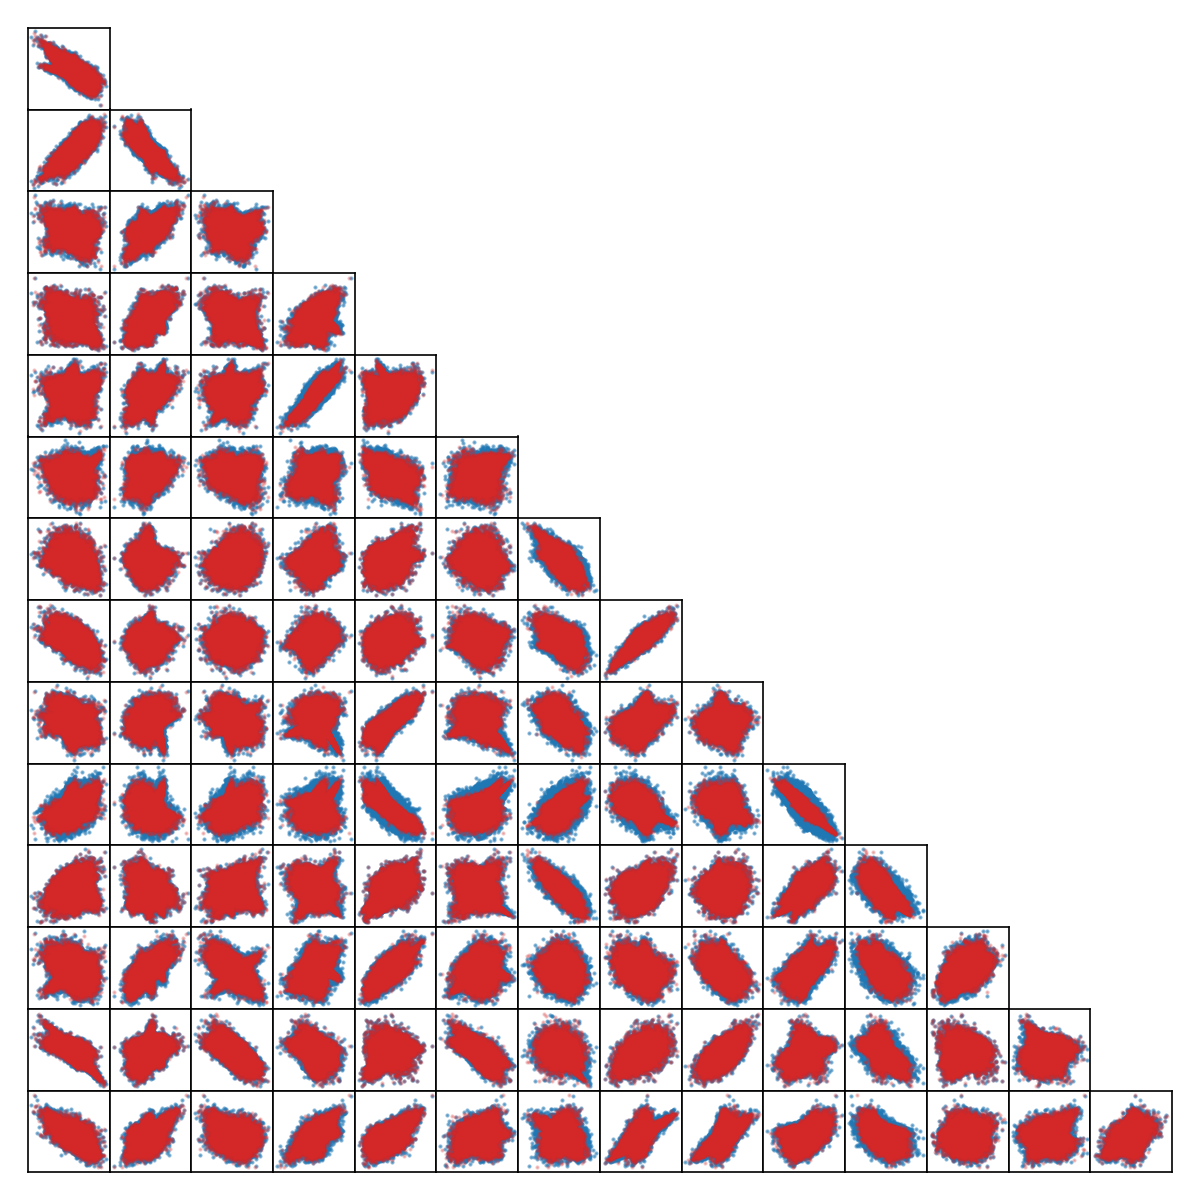
\includegraphics[width=1.0\textwidth]{experiments/toy-model-data.png}
    \caption{A corner plot showing all $\NumDimensions$ dimensions of the
    		 generated data for Experiment~1 (blue). Overplotted in red
		 	 we show samples generated given our estimate of the model 
			 parameters, without adding specific variance in each dimension.
			 This demonstrates that the model parameters estimated by
			 expectation-maximization can replicate the generated data.}
    \label{fig:toy-model-data}
\end{figure*}


\begin{figure*}
	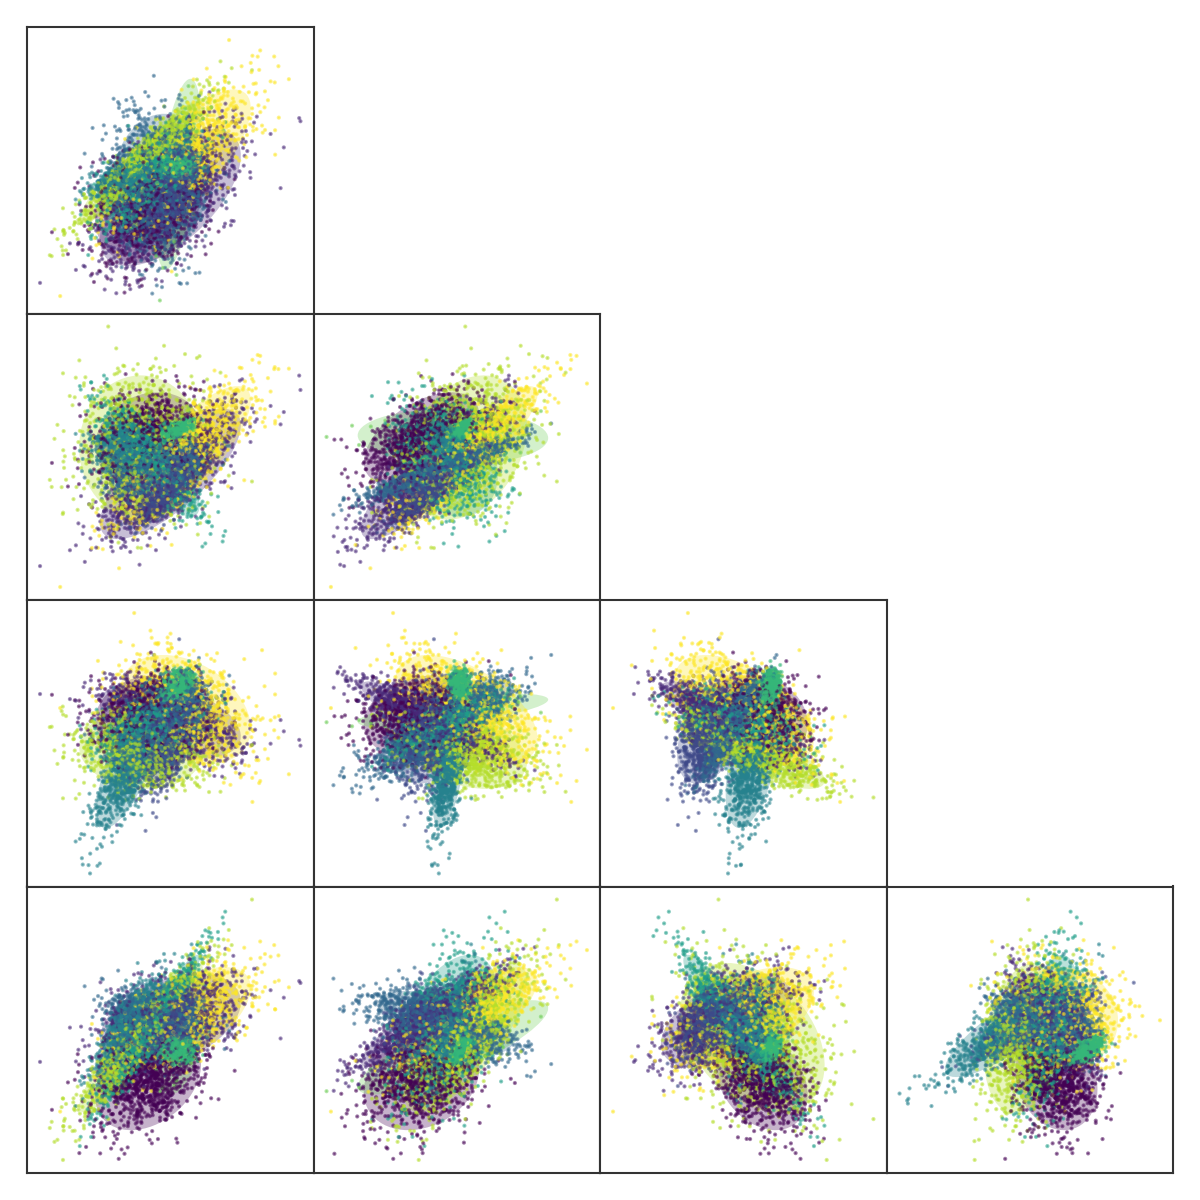
\includegraphics[width=1.0\textwidth]{experiments/toy-model-latent-space.png}
    \caption{A corner plot showing all $\NumLatentFactors$ dimensions in
    		 latent space, where each data point is coloured by the component
		 	 that it is estimated to belong to.}
    \label{fig:toy-model-latent-space}
\end{figure*}




\subsubsection{Model fitting given the true number of latent factors and components}

We initialised the factor loads and component assignments randomly, and
fit this generated data set using the expectation-maximization algorithm
as described in the previous Section. After 58 iterations
(and a serial processing time of 40 seconds) we
reached our convergence threshold: the log probability increased by
less than $10^{-5}$ with each iteration (\todo{Figure~X}). For this experiment we specified
the number of latent factors $\NumLatentFactors$ and the number of clustering components
$\NumComponents$ to include, but below we repeat this experiment where the number
of latent factors and clustering components is not known.

\begin{figure}
	%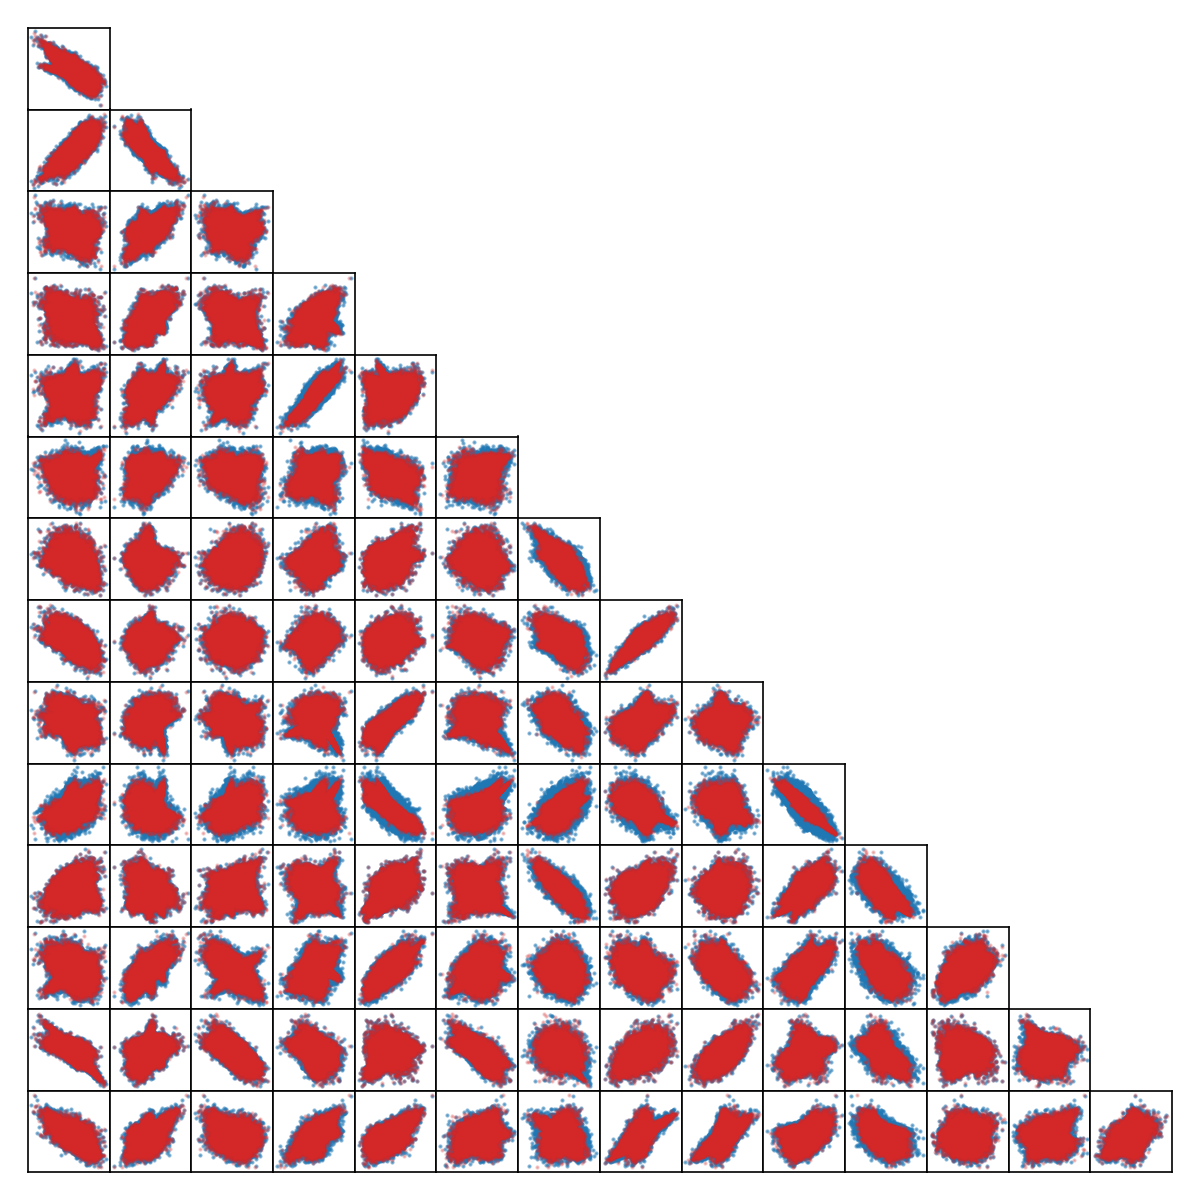
\includegraphics[width=0.5\textwidth]{experiments/toy-model-data.png}
    \caption{Log-likelihood of the model given the data $\mathcal{L}\left(\vec\data|\vec\Psi\right)$ for Experiment 1 as a function of the number of expectation-maximization iterations. After \todo{X} iterations the improvement in log-likelihood per
    expectation-maximization cycle was less than $10^{-5}$.}
    \label{fig:toy-log-likelihood-per-iteration}
\end{figure}


We show a corner plot of the data in Figure~\ref{fig:toy-model-data}.
In this figure we have over-plotted 100000 samples generated by the
estimated factor loads $\factorloads_\textrm{est}$ and the clustering in factor 
scores $\scoremeans_\textrm{est}$ and $\scorecovs_\textrm{est}$ (weighted by $\vec\weight_\textrm{est}$)
-- without adding variance $\specificvariance_\textrm{est}$ % Ref Factor load figure 
-- in order to illustrate that the
estimated model parameters can realistically generate the data.
The estimated latent space of factor scores is shown in 
Figure~\ref{fig:toy-model-latent-space} where the colours indicate the
most likely component that the data point is associated with.

While the estimated model parameters can generate the data and demonstrate
clustering in latent space, caution is needed when interpreting the 
model latent variables.
Latent factor models are by definition indeterminate in that there are
multiple solutions of the parameter vector $\vec\Psi$ which provide
an identical data-generating process. This can be trivially shown by
the fact that the factors loads and scores can be rotated by taking the
dot product
with some rotation
matrix $\textbf{R}$ and generate the exact same data. As a consequence,
we cannot strictly evaluate our model fitting procedure by comparing
how closely the inferred factor loads (or scores) match the true 
variables. This is further complicated by orientation and order
of the latent factors: even if the inferred factor loads were very close
to the true factor loads, they could be ordered differently, or have
their signs reversed. We discuss this further in later sections.

\subsubsection{A grid search for the number of latent factors and components}

Here we treat the generated data set as if the true number of latent factors
and the true number of components are not known. Starting with $\NumLatentFactors = 1$
and $\NumComponents = 1$, we trialled each permutation of $\NumLatentFactors$ and $\NumComponents$
until $\NumLatentFactors_{max} = 10$
and   $\NumComponents_{max} = 40$ (e.g., twice $\NumLatentFactors_{true}$ and $\NumComponents_{true}$).
For each $\NumLatentFactors,\NumComponents$ permutation we initialised the factor
loads and component assignments randomly. We performed expectation-maximization 
cycles until the relative log-likelihood improved by less than $10^{-5}$. We then
recorded the log-likelihood of the data given the model parameters, the
Bayesian Information Criterion \citep{bic}, 
\begin{equation}
	\textrm{BIC} = Q\log{N} - 2\log\mathcal{L}\left(\data|\vec\Psi\right) \label{eq:bic}
\end{equation} 
\noindent{}and the pseudo-Bayesian Information Criterion \citep{pseudo-bic}
\begin{equation}
 \textrm{pseudo-BIC} = 6(1 + \gamma)\omega{}Q\log{N} - 2\log\mathcal{L}\left(\data|\vec\Psi\right) \label{eq:pseudo-bic}
\end{equation}
\noindent{}where $Q$ is the total number of model parameters in both equations,
and the unknown constants $\omega$ and $\gamma$ have constraints
$\omega \geq 1$ and $\gamma > 0$. Here we adopt $\gamma = 0.1$ and $\omega = 1$.
These metrics are shown in Figure~\ref{fig:experiment-1-gridsearch}.



\begin{figure}
	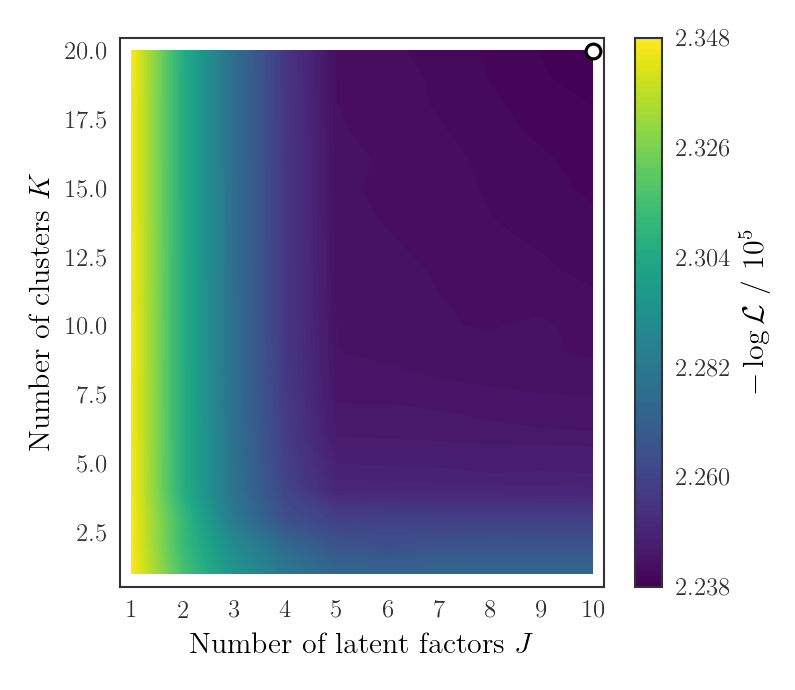
\includegraphics[width=0.45\textwidth]{experiments/toy-ll-contours.png}
	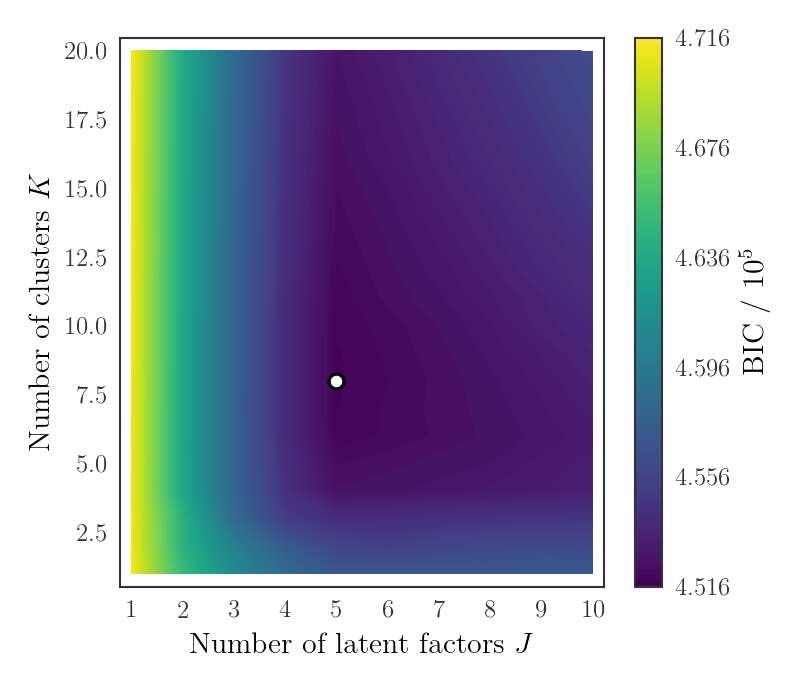
\includegraphics[width=0.45\textwidth]{experiments/toy-bic-contours.png}
	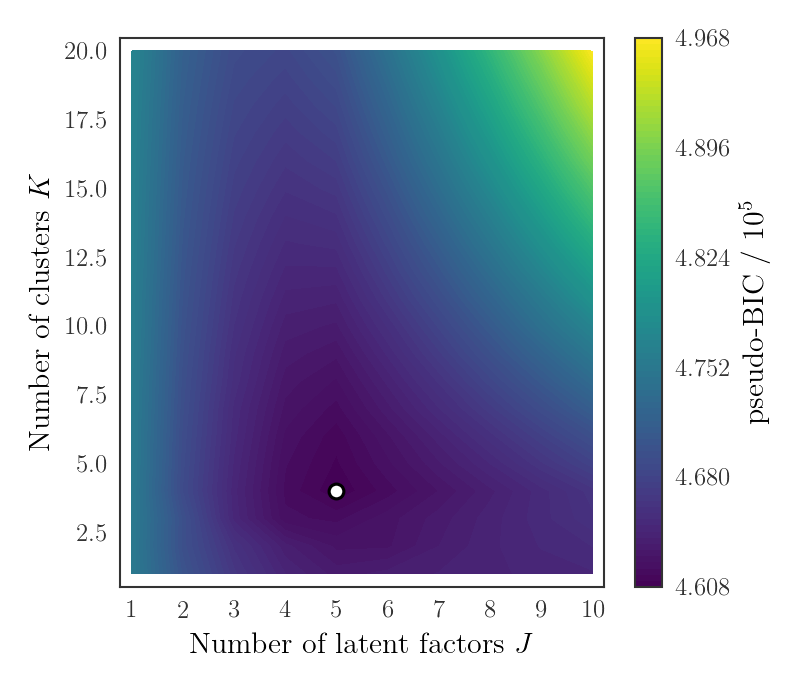
\includegraphics[width=0.45\textwidth]{experiments/toy-pseudobic-contours.png}
    \caption{Model performance metrics resulting from a gridsearch using the
    		 data generated as part of our toy model. The top 
		 	 panel shows the negative log-likelihood 
			 $-\log{\mathcal{L}\left(\data|\vec\Psi\right)}$ 
			 evaluated at each combination of latent factors $J$ and number 
			 of clusters $K$, the middle panel shows the BIC (Equation \ref{eq:bic}), 
			 and the lower panel shows
			 the pseudo-BIC
			 (Equation~\ref{eq:pseudo-bic}). The marker indicates the 
			 lowest value in each panel.}
    \label{fig:experiment-1-gridsearch}
\end{figure}




Unsurprisingly the log likelihood increases with increasing numbers of latent
factors $\NumLatentFactors$ and increasing numbers of components $\NumComponents$.
The lowest BIC value is found at $\NumLatentFactors = 5$
and $\NumComponents = 8$, close to the true values ($\NumLatentFactors_{true} = 5$,
$\NumComponents_{true} = 10$). The lowest pseudo-BIC value is also found at
$\NumLatentFactors = 5$, but with fewer components: $\NumComponents = 4$.

The estimated latent factor loads found during this grid search are shown in
Figure~\ref{fig:fig:experiment-1-gridsearch-factors-init-random-and-random},
where each panel shows the estimated latent factor loads found by
expectation-maximization for a given number of latent factors and components.
The latent factors $\factorloads$ in each panel are multiplied by a rotation
matrix $\mathbf{R}$ with entries $\{-1, 0, 1\}$ in order to re-orient and flip
the estimated latent factors to be as similar as possible to the latent factors
found from the model with the same number of latent factors and $\NumComponents  =  1$.
In doing so we find that the estimated latent factors vary slightly as
the number of components $\NumComponents$ increases, but the overall shape
of the latent factors remains the same.


\begin{figure*}
	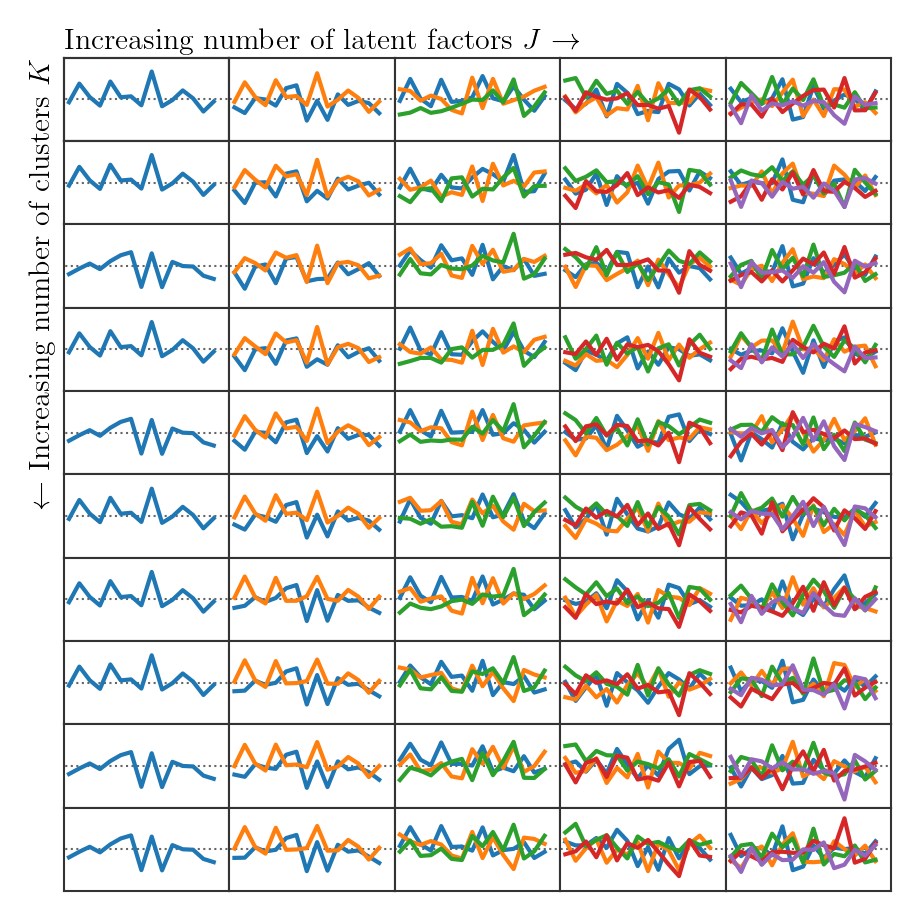
\includegraphics[width=1.0\textwidth]{experiments/toy-factors-init-randomly.png}
	\caption{Latent factor loads inferred for models with increasing numbers
			 of latent factors and increasing numbers of cluster components
			 in Experiment~1, where the latent factors and component assignments
			 were initialised randomly.
				The top left panel shows the results of the model with
			 $\NumLatentFactors = 1$ and $\NumComponents = 1$. 
			 The latent factors in each panel have been rotated by a
			 rotation matrix $\textbf{R}$ with entries $\{-1, 0, +1\}$ such 
			 that the estimated latent factors in each model are ordered 
			 and oriented to be as similar as the latent factors estimated from
			 the model with only one component (i.e., the latent factors in the top row
			 of the same column). Note that the rotation
			 matrix contains only entries $\{-1, 0, +1\}$.}
	\label{fig:toy-factors-init-randomly}
\end{figure*}

\todo{This structure goes away and becomes more consistent if we change the initialisation
procedure}

\todo{figure of toy factors init svd kmeans++}

\todo{log-likelihood of different initialisation routines}



\begin{figure*}
	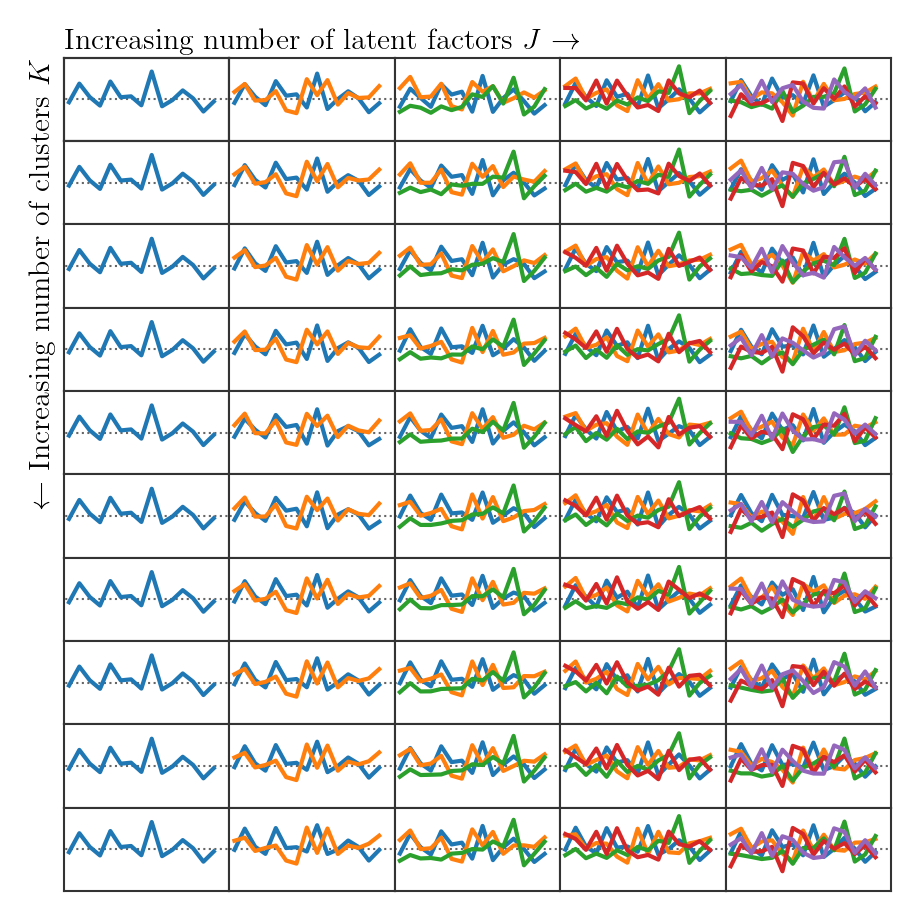
\includegraphics[width=1.0\textwidth]{experiments/toy-svd-kmeans-factors.png}
	\caption{Latent factor loads inferred for models with increasing numbers
			 of latent factors and increasing numbers of cluster components
			 in Experiment~1, where the latent factors were initialised using
			 \texttt{SVD} and the component assignments were initialised using \texttt{k-means++}.
				The top left panel shows the results of the model with
			 $\NumLatentFactors = 1$ and $\NumComponents = 1$. 
			 The latent factors in each panel have been rotated by a
			 rotation matrix $\textbf{R}$ with entries $\{-1, 0, +1\}$ such 
			 that the estimated latent factors in each model are ordered 
			 and oriented to be as similar as the latent factors estimated from
			 the model with only one component (i.e., the latent factors in the top row
			 of the same column). Compared to Figure~\ref{fig:toy-factors-init-randomly},
			 it is clear that initialising with \texttt{SVD}/\texttt{k-means++} results
			 in less scatter in the final estimates of the model parameters.}
	\label{fig:toy-factors-init-svd-and-kmeans++}
\end{figure*}

The results of this experiment confirm that the model is indeterminate, in 
that there are multiple equally valid solutions that can exactly reproduce
the data. It also highlights the importance of initialisation, demonstrating
how the initialisation of the common latent factors can impact the final
model parameters. These two points are related, as one could initialise the
latent factors randomly (or from noise) and multiply that model with a
rotation matrix $\mathbf{R}$ that rotates the latent space such that the
common factor loads are aligned closer to some prior expectation that we have
for the common factor loads (e.g., in that they should represent plausible
astrophysical yields). Motivated by these results and indeterminate nature
of the model, in Experiment~2 we initialise the common factor loads
to represent known astrophysical processes such that they can be interpreted
in context with the data.


\subsection{Experiment 2: A minimal set of nucleosynthetic trace elements in \Galah}

In this experiment we further investigate the effects of initialising the model parameters.
Here we make use of a minimal set of nucleosynthetic trace elements
using the second \Galah\ data release \citep{Buder:2018}. Specifically, we use
reliable chemical abundance measurements of Na (an odd-Z element), Mg and Ca (alpha-elements),
Ni, Fe, and Cr (iron-peak elements), Ba and Y (s-process tracers), and Eu (an r-process tracer).
We assume that there are four latent factors ($J = 4$) and four components ($K = 4$),
and we initialise the latent factors and component parameters in different combinations.

To initialise the latent factors using astrophysical insight (or domain expertise)
we make the following steps:
\begin{enumerate}
	\item We initialise all entries of $\factorloads$ to be drawn from $\mathcal{N}\left(0, 10^{-2}\right)$.
	\item For the first latent factor we set the entries that correspond to Ni, Fe, and Cr to be $+1$ (e.g., Fe-peak).
	\item For the second latent factor we set the entries that correspond to Mg and Ca to be $+1$ (e.g., $\alpha$-elements).
	\item For the third latent factor we set the entries that correspond to Ba and Y to be $+1$ (e.g., the s-process).
	\item For the fourth latent factor we set the entry that corresponds to Eu to be $+1$ (e.g., the r-process).
\end{enumerate}


%The latent factors can be initialised in four different ways: (1) with entries drawn randomly from $\mathcal{U}\left(-1, +1\right)$, (2) with noisey draws $\mathcal{N}\left(0, 10^{-2}\right)$, (3) using singular value decomposition, and (4) using astrophysical insight to initialise the factor loads. 

The component parameters are either initialised randomly, or using \texttt{K-means++} algorithm in
the latent space given the initial estimate of the latent factors. For each combination of 
initialisation procedure, we run 30 optimisations and record the log likelihood once the E-M 
procedure has reached a threshold of $10^{-8}$.
The results of this experiment are shown in Figure~\ref{fig:experiment-4-log-L}.
In most cases the final log likelihood is within the threshold of $10^{-8}$ between
different optimisation runs of the same initialisation procedure. However, it is clear
that at least some initialisations result in a local optimum, emphasising the importance in
optimising from many initialisations. 

Figure~\ref{fig:experiment-4-log-L} demonstrates that even though the initialisation procedure
can impact the final estimate of the model parameters, the resulting log likelihood values
are within the convergence threshold. This is, again, a consequence of the indeterminate
nature of the model specification. However, the advantage here is that these results
demonstrate that we \emph{can} initialise the latent factors with domain knowledge,
without a significant detriment to the final log likelihood. Similarly, in Figure~\ref{fig:experiment-4-astrophysical-latent-factors}
we show that the initial latent factors are indeed different from the final latent factors,
and that there is some variance in our estimates of the latent factors from 30 initialisations.
\todo{something to say here about not biasing our results?}

The results from this experiment demonstrate that we can initialise the latent factors
using domain knowledge without incurring strong biases in our final estimates of the
latent factors, or introducing a significant detriment to the log likelihood, as long
as we initialise the model many (e.g., $\gtrsim 5$) times.

\begin{figure}
	\includegraphics[width=0.5\textwidth]{experiments/galah-experiment-4-log-L-hist.png}
	\caption{Log likelihoods $\mathcal{L}\left(\data|\vec\Psi\right)$ of optimised
			 models using \Galah\ data in Experiment 4 with four latent factors
			 and four components ($J = 4$, $K = 4$). The columns indicate different
			 methods to initialise the component parameters ($\pi$, $\scoremeans$,
			 $\scorecovs$), and the rows represent different methods to initialise
			 the latent factors ($\factorloads$). Each combination of initialisation
			 procedure has 30 models where E-M was run until a threshold of $10^{-8}$
			 was reached in $\log{L}$.}
	\label{fig:galah-experiment-4-log-L}
\end{figure}


\todo{experiment-4-astrophysical-latent-factors}


\subsection{Experiment 3: A subset of gravitationally bound stellar clusters from \Galah\ and elsewhere}
\label{sec:experiment-galah-clusters}



\subsection{Experiment 4: A subset of 14 chemical abundances in \Galah}
\label{sec:experiment-galah}


We use the second \Galah\ data release \citep{Buder:2018a} which
includes up to 23 chemical abundances measured for 342,682
stars. It is not practical to use all of these measurements as-is
when performing chemical tagging. For example, our experiments
with \Galah\ data do not include lithium abundances because the
photospheric lithium varies throughout a star's lifetime. 
We first selected stars with \texttt{flag\_cannon = 0} to exclude
stars where there is reason to suspect that the stellar parameters
(e.g., $\teff$, $\logg$) are unreliable, and as a result the 
detailed chemical abundances are untrustworthy. 

We included the following fourteen chemical abundances: Na, Mg, 
Si, Ca, Sc, Ti, Cr, Mn, Fe, Ni, Cu, Zn, Ba, and Eu.
By requiring that each star has \texttt{flag\_cannon = 0} and
\texttt{flag\_<x> = 0} (where \texttt{<x>} is the relevant label)
for each chemical abundance, this leaves
us with a sample of 12,798 stars each with reliable stellar
parameters ($\teff$, $\logg$) and chemical abundances.
This is relevant to the approach we use here, as the method
described here requires no missing data.
These elements are produced from multiple nucleosynthetic
pathways, and it is this subsample that we will use for 
our initial chemical experiment with \Galah\ data.




%\subsubsection{Search strategy} \label{sec:experiment-galah-search}

The expectation-maximization procedure outlined in Section \ref{sec:methods} describes 
the process of refining our estimate of the model parameters $\vec\psi$ until
the improvement in log probability between iterations decreases below some
pre-defined threshold. This method is valid for a pre-defined number of latent
factors, and a pre-defined number of components to cluster in latent space.
In practice these values are not known. For the purposes of this work, we 
perform a grid-based search in $J$ and $K$, perform E-M for each combination of
$J$ and $K$, and record the optimal parameters.

We trial the number of latent factors from $J = 1$ to $J = 12$, and trial the
number of clustering components from $K = 1$ to $K = 40$. We re-initialise the
mixture for each new trial of $\{J, K\}$, and do not make use of results from
`nearby' mixtures. After the E-M threshold of $10^{-5}$ has been reached, we
record the log likelihood of the data given the model parameters, the
Bayesian Information Criterion \citep{bic}, 
\begin{equation}
	\textrm{BIC} = Q\log{N} - 2\log\mathcal{L}\left(\data|\vec\Psi\right) \label{eq:bic}
\end{equation} 
\noindent{}and the pseudo-Bayesian Information Criterion \citep{pseudo-bic}
\begin{equation}
 \textrm{pseudo-BIC} = 6(1 + \gamma)\omega{}Q\log{N} - 2\log\mathcal{L}\left(\data|\vec\Psi\right) \label{eq:pseudo-bic}
\end{equation}
\noindent{}where $Q$ is the total number of model parameters in both equations,
and the unknown constants $\omega$ and $\gamma$ have constraints
$\omega \geq 1$ and $\gamma > 0$. Here we adopt $\gamma = 0.1$ and $\omega = 1$.


\todo{Discuss grid search, inferred factor loads, cluster variances, etc.}



\begin{figure}
	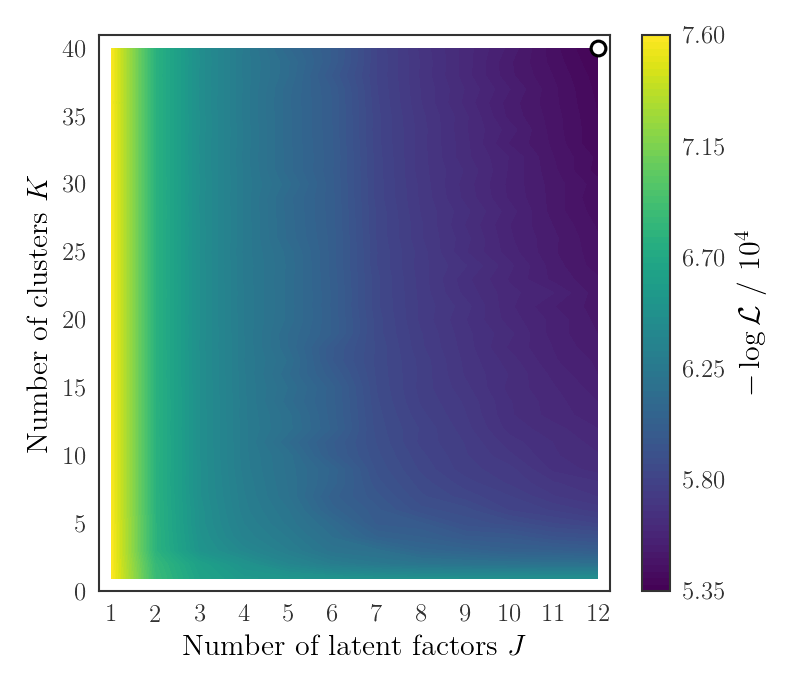
\includegraphics[width=0.45\textwidth]{experiments/galah-experiment-2-gridsearch-ll-contours.png}
	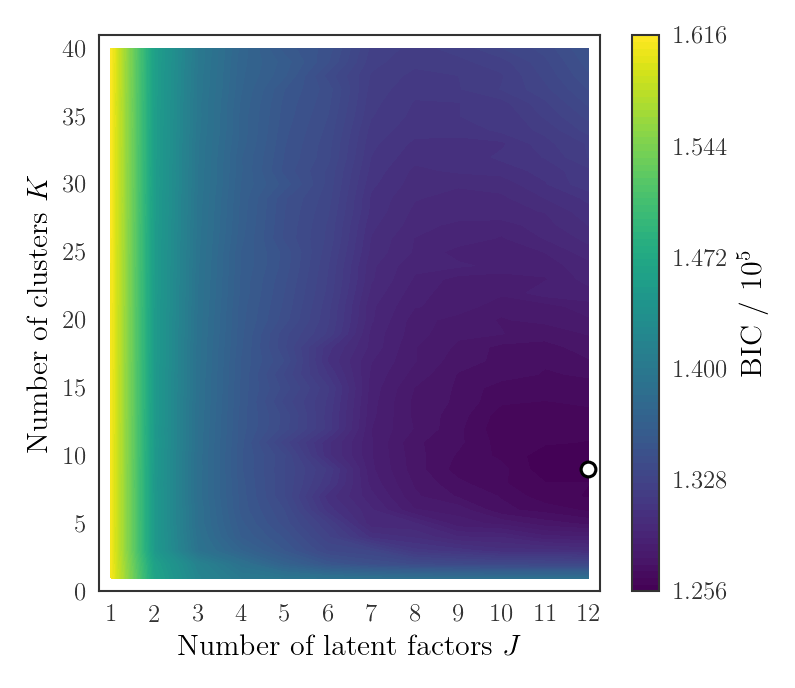
\includegraphics[width=0.45\textwidth]{experiments/galah-experiment-2-gridsearch-bic-contours.png}
	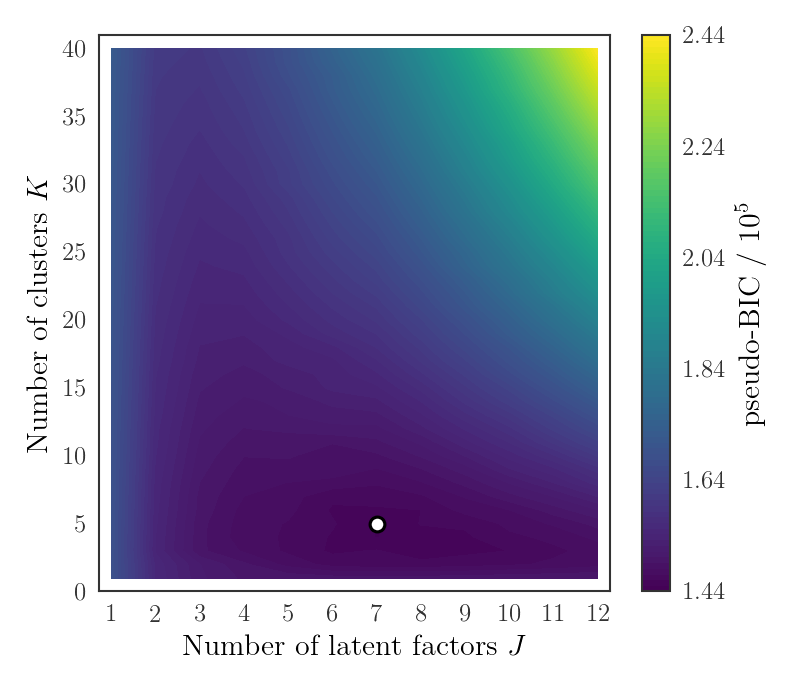
\includegraphics[width=0.45\textwidth]{experiments/galah-experiment-2-gridsearch-pseudobic-contours.png}
    \caption{Model performance metrics for Experiment 2 using a subset of 14 
    		 \Galah\ chemical abundances measured from 12,798 stars. The top 
		 	 panel shows the negative log-likelihood 
			 $-\log{\mathcal{L}\left(\data|\vec\Psi\right)}$ 
			 evaluated at each combination of latent factors $J$ and number 
			 of clusters $K$, the middle panel shows the Bayesian Information
			 Criterion (Equation \ref{eq:bic}), and the lower panel shows
			 the pseudo-Bayesian Information Criterion 
			 (Equation~\ref{eq:pseudo-bic}). The white marker indicates the 
			 lowest value in each panel.}
    \label{fig:experiment-2-gridsearch}
\end{figure}

\begin{figure*}
	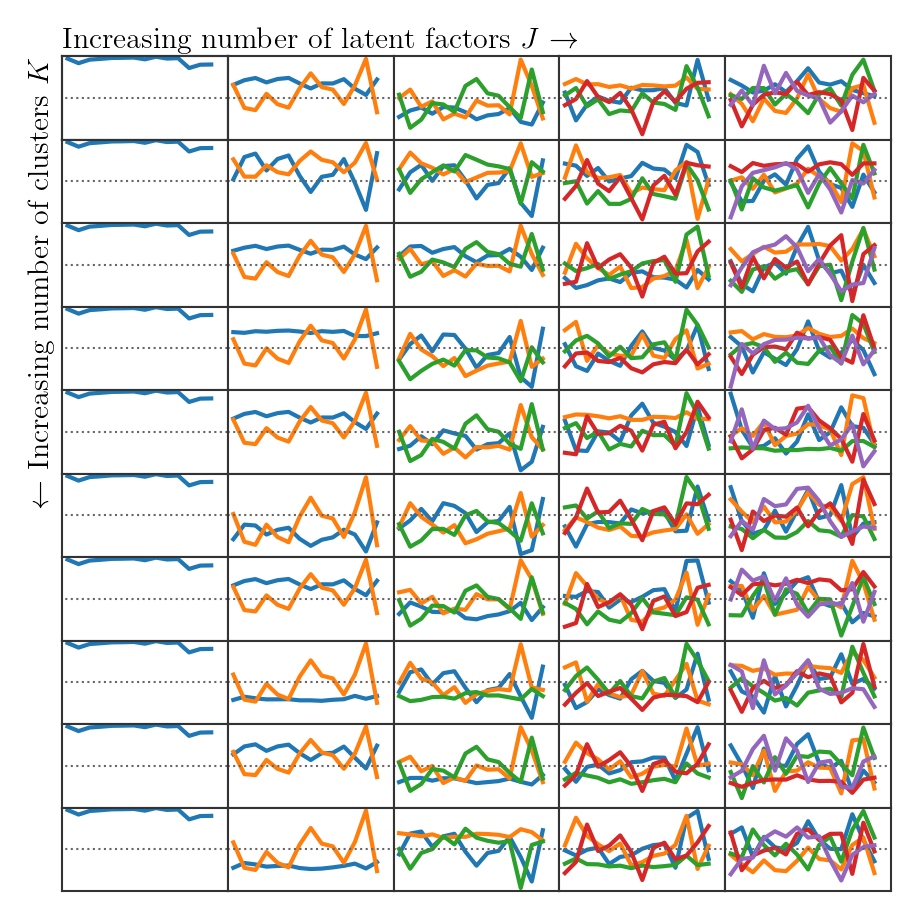
\includegraphics[width=1.0\textwidth]{experiments/galah-experiment-2-gridsearch-factors-wrt-J-and-K.png}
	\caption{Latent factor loads inferred for models with increasing numbers
			 of latent factors and increasing numbers of cluster components
			 in Experiment~2. The latent factors have each been rotated by a
			 rotation matrix $\textbf{R}$ with entries $\{-1, 0, +1\}$ such 
			 that the estimated latent factors in each model are ordered 
			 and oriented to be as similar as the latent factors estimated from
			 the model with only one latent factor. Note that the rotation
			 matrix contains only entries $\{-1, 0, +1\}$. The latent
			 factors for each model shown here were initialised randomly.
			 }
	\label{fig:experiment-2-gridsearch-factors-init-svd}
\end{figure*}






\section{Results} \label{sec:results}

\section{Discussion} \label{sec:discussion}

\section{Conclusions} \label{sec:conclusion}

\acknowledgements
A.~R.~C. is supported in part by Australian Research Council
Discovery Project DP160100637.
% Gaia acknowledgement?
% GALAH acknowledgement?

\software{
	\package{Astropy} \citep{astropy:v1,astropy:v2},
    \package{IPython} \citep{ipython},
    \package{matplotlib} \citep{mpl},
    \package{numpy} \citep{numpy},
    \package{scipy} \citep{scipy},
    \package{Stan} \citep{stan},
    \package{Jupyter Notebooks} \citep{jupyter-notebooks}
}    

\appendix

\section{Nomenclature}\label{app:symbols}

\todo{summarise symbols}

\bibliographystyle{aasjournal}
\bibliography{mcfa}

\end{document}
